\documentclass[a4paper]{oblivoir}
% define the title
\author{Moon Il-chul \\ \href{mailto:icmoon@kaist.ac.kr}{icmoon@kaist.ac.kr} 
   \and Hwang Gyeong-jo
 \\ \href{mailto:hkj4276@kaist.ac.kr}{hkj4276@kaist.ac.kr} }
 \setcounter{chapter}{4}
\title{Chapter 4. Logistic Regression}
\usepackage{indentfirst}
\usepackage{graphicx}
\graphicspath{ {Figure/} }
\usepackage{hyperref}
\usepackage{amsmath}
\usepackage{amssymb}
\usepackage{amsfonts}
\usepackage{dsfont}
\usepackage[]{algorithm2e}
\usepackage{chngcntr}
\counterwithin{figure}{chapter}
\setcounter{tocdepth}{2}
\setcounter{secnumdepth}{3}
\hypersetup{pdfborder={0 0 0}}
\renewcommand{\thefigure}{\thechapter-\arabic{figure}}
\renewcommand{\theequation}{\thechapter.\arabic{equation}}
\newlength\myindent
\setlength\myindent{5em}

\begin{document}
% generates the title
\maketitle
%\renewcommand{\contentsname}{목차}
\tableofcontents
%\listoftables
%\listoffigures

%슬라이드 2
\section*{}
2단원에서는 규칙기반, 의사결정 나무, 선형회귀 등의 고전적인 방법에 대해 배웠고, 지난 3단원에서는 Naive Bayes Classifier에 대해 공부해보았다. Naive Bayes 방법은 본질적으로 조건부 독립을 적용한 MLE, MAP와 같다는 것을 상기하자. 이 단원에서는 Naive Bayes Classifier의 전제 조건인 Naive 가정을 하지 않고 학습할 수 있는 방법론을 배워볼 것이다.

%슬라이드 3
\section{Logistic Regression}

%슬라이드 4
\subsection{Optimal Classification and Bayes Risk}
\begin{figure}[ht]
\centering
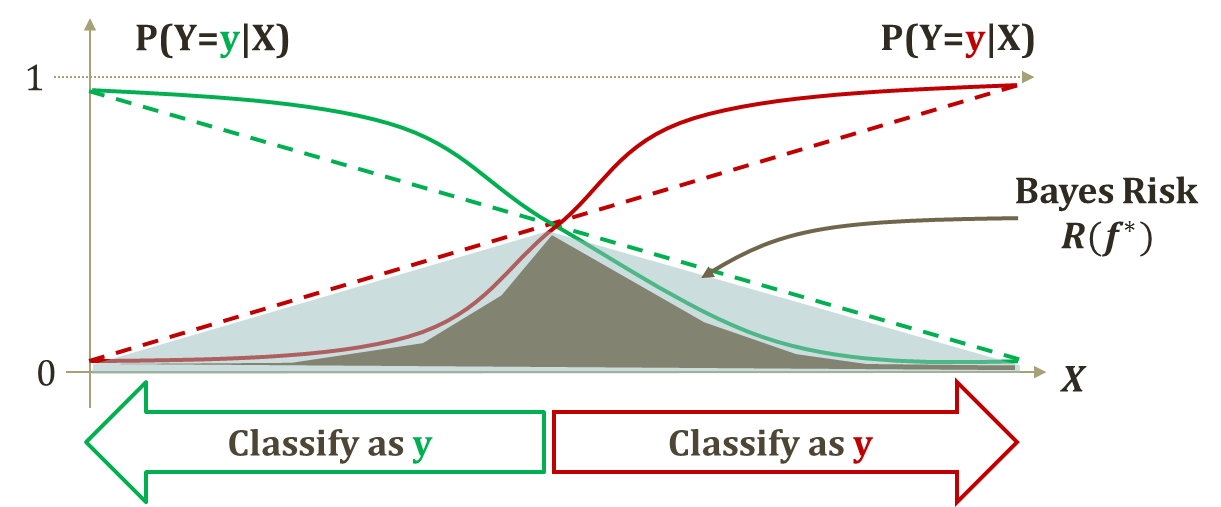
\includegraphics[scale=0.6]{Bayes_Risk.png}
\caption{조건부 확률 그래프와 베이즈 위험}
\label{Figure 4-1}
\end{figure}

\indent 위의 그래프는 이전 단원에서 본 것과 동일하다. x축은 독립변수인 $x$의 값을 나타내고, y축은 해당 $x$값이 주어졌을 때의 종속변수 $y$의 조건부 확률을 나타낸다. 하늘색 영역이 점선 형태의 확률밀도함수를 이용했을 때, 진녹색 영역이 곡선 형태의 확률밀도함수를 이용했을 때 잘못 분류할 확률을 나타낸 부분이다. 이 위험(Risk)을 베이즈 위험(Bayes Risk)이라고 정의하였다. 그래프의 점선처럼 직선 형태의 확률분포보다는 실선의 곡선 형태 확률분포가 베이즈 위험의 영역이 적으므로 우리가 활용하기에 더 좋은 형태의 함수라고 할 수 있다. 가운데 두 직선(또는 곡선)들이 만나는 지점을, Class Variable에 대한 예측값이 달라진다는 의미에서 결정 경계(Decision Boundary)라고 부른다. \\
\indent 흔히 통계학에서 사용하는 Probit 모델 또는 Multinomial Probit 모델에서는 조건부 확률을 선형함수(Linear Function)로 가정하지 않는다. 그 이유는 추정된 매개변수로 함수를 만들었을 때, 종속변수 $x$의 값에 따라 확률이 0$\sim$ 1 사이를 벗어나는 경우가 있기 때문이다. 또한 미분값이 항상 일정하므로, 최적화 기법을 사용하기에 적절치 않다는 이유도 있다. 이 그래프 예시에서도 마찬가지의 이유로 선형함수보다는 곡선형태의 함수를 더 선호한다. 따라서, 우리는 조건부 확률밀도함수(Conditional Probability Density Function)를 다음과 같은 \textbf{S자형 곡선}으로 가정할 필요가 있다. \\
\begin{figure}[ht]
\centering
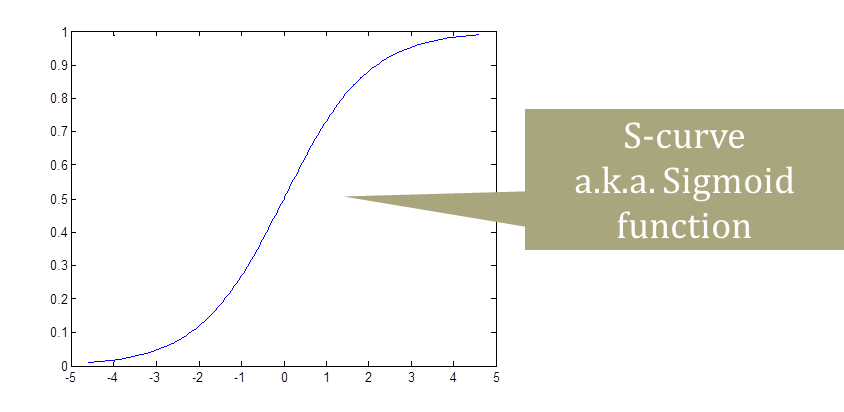
\includegraphics[scale=0.6]{Bayes_Risk2.png}
\caption{S-curve or Sigmoid function}
\label{Figure 4-2}
\end{figure}

%슬라이드 5
\subsection{Dataset: UCI 신용평가 데이터}
이 단원에서 사용할 방법론들은 지난 2단원에서 사용했던 UCI 신용평가 데이터에 적용해 볼 것이다. 이 데이터에서 모든 항목(Attribute)명은 고객의 개인정보 보호를 위해 A1 $\sim$ A15와 같이 변환되었다. (각 항목의 값 역시 비슷한 형태로 변형되었다.) 여기서 A2, A3, A8, A11, A14, A15 등 6개 항목은 값이 연속적인(Continuous) 변수이고, 나머지는 모두 이산적인(Discrete) 변수이다. C는 신용평가 결과가 +(신용대출 허가) 인지, -(신용대출 불허) 인지를 나타내는 Class 변수임을 상기하자. \\
\begin{figure}[ht]
\centering
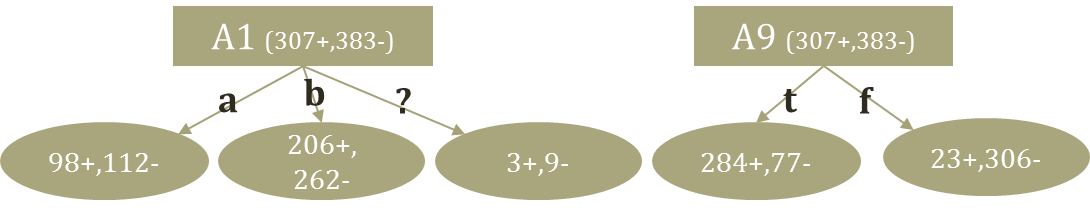
\includegraphics[scale=0.6]{UCI_Data.png}
\caption{UCI 신용평가 데이터 - A1과 A9으로 분류한 결과}
\label{Figure 4-3}
\end{figure}

\begin{itemize}\itemsep0pt
\item A1: a, b
\item A2: Continuous
\item A3: Continuous
\item A4: u, y, l, t
\item A5: g, p, gg
\item A6: c, d, cc, i, j, k, m, r, q, w, x, e, aa, ff
\item A7: v, h, bb, j, n, z, dd, ff, o
\item A8: Continuous
\item A9: t, f
\item A10: t, f
\item A11: Continuous
\item A12: t, f
\item A13: g, p, s
\item A14: Continuous
\item A15: Continuous
\item C: +, -
\end{itemize}

%슬라이드 6
\subsection{하나의 변수를 이용한 분류}
Class Variable의 대출허가는 1, 불허는 0의 값으로 바꾸고 이를 아래 그래프의 y축에 나타내었다. 그래프의 x축은 우리가 변화시킬 수 있는 독립변수로서, A15에 해당하는 Attribute Variable을 사용하였다. A15는 연속적인 변수임을 상기하자. \\
\begin{figure}[ht]
\centering
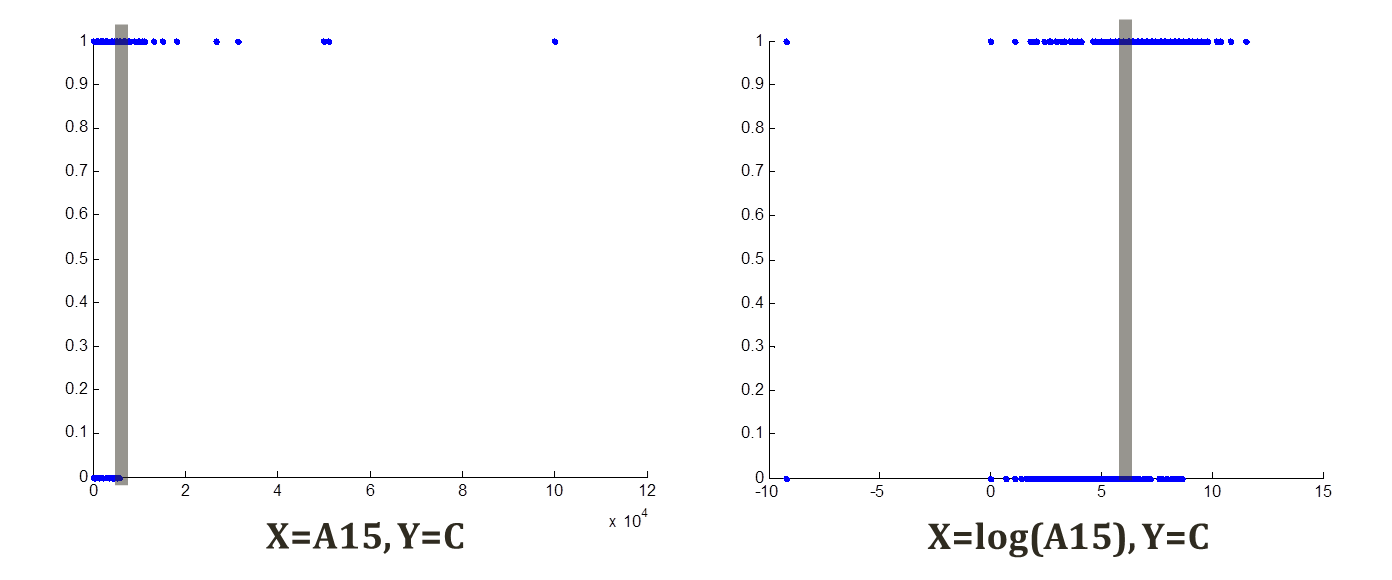
\includegraphics[scale=0.6]{Classification_1_Variable.png}
\caption{A15 하나의 변수와 Class Variable 사이의 그래프}
\label{Figure 4-4}
\end{figure}

\indent 왼쪽의 그래프를 먼저 살펴보면 $C=0$일 때, 즉 신용대출 불허가 났을 때의 A15의 값은 회색 선 왼쪽에 모두 몰려있는 것을 볼 수 있다. $C=1$일 때에는 이전과 마찬가지로 낮은 값의 A15도 있지만, 회색 선 오른쪽의 비교적 큰 값을 가지는 데이터도 있음을 확이할 수 있다. 이번에는 A15값에 로그를 취하여 x축에 나타낸 오른쪽 그래프를 살펴보자. 로그를 취함으로써 우리는 A15 변수의 지수함수적 변화를 선형함수로 치환하여 변화율을 낮추는 효과를 얻을 수 있다. 그림에서 다음과 같은 회색 선을 그엇을 때, (물론 이 기준이 정확하게 신용대출 허가/불허를 나누지는 않지만) 대출 허가를 받은 사람들이 비교적 큰 x값을, 불허를 받은 사람들이 비교적 작은 x값을 가짐을 알 수 있다. 우리는 각각의 Attribute Variable 별로 어떤 값을 기준으로 나누었을 때, 신용대출 허가를 받을 확률이 얼마인지를 알 필요가 있다.

%슬라이드 7
\subsection{선형함수 vs 비선형함수}
다음의 그림에서 왼쪽 그래프는 x값이 A15 변수의 값을 그대로 가져온 것이고, 오른쪽 그래프는 이전 슬라이드와 같이 x값을 로그함수로 압축하여 그린 것이다. y값은 이전과 다르게 class 값을 그대로 가져오는 것이 아니라, x값이 주어졌을 때 class 값이 1인 조건부 확률을 계산하여 나타내었다. 파랑 점들은 실제 관측값이 발생한 지점들, 즉 데이터의 위치를 나타낸 것이고, 빨강 점들은 선형회귀를 이용하여 함수의 그래프를 추정했을 때 각각의 x값 마다 해당하는 y의 위치를 나타낸 것이다. 초록 점들은 이 단원에서 배우고자 하는 로지스틱(Logistic) 회귀를 이용하여 함수의 그래프를 추정한 결과이다. \\
\indent 빨강 점들을 보면 선형회귀의 결과가 확률의 범위인 0 $\sim$ 1 사이를 벗어나는 것을 관찰할 수 있다. 앞서 말한 Probit 모델에서 조건부 확률을 선형함수로 추정하지 않는다는 것을 상기하자. 로지스틱 함수는 그림에서와 같이 S자형 곡선의 형태를 띠는 것을 확인할 수 있다. 오른쪽 그래프에서 황갈색 선은 회귀 방정식의 결과, 확률을 0.5로 반반 나누는 지점을 나타낸 것인데, 어림짐작으로 알 수 있듯이 초록색 점들이 나눈 기준인 왼쪽 선이 좀 더 바람직한 분류 기준이 될 것이다.
\begin{figure}[ht]
\centering
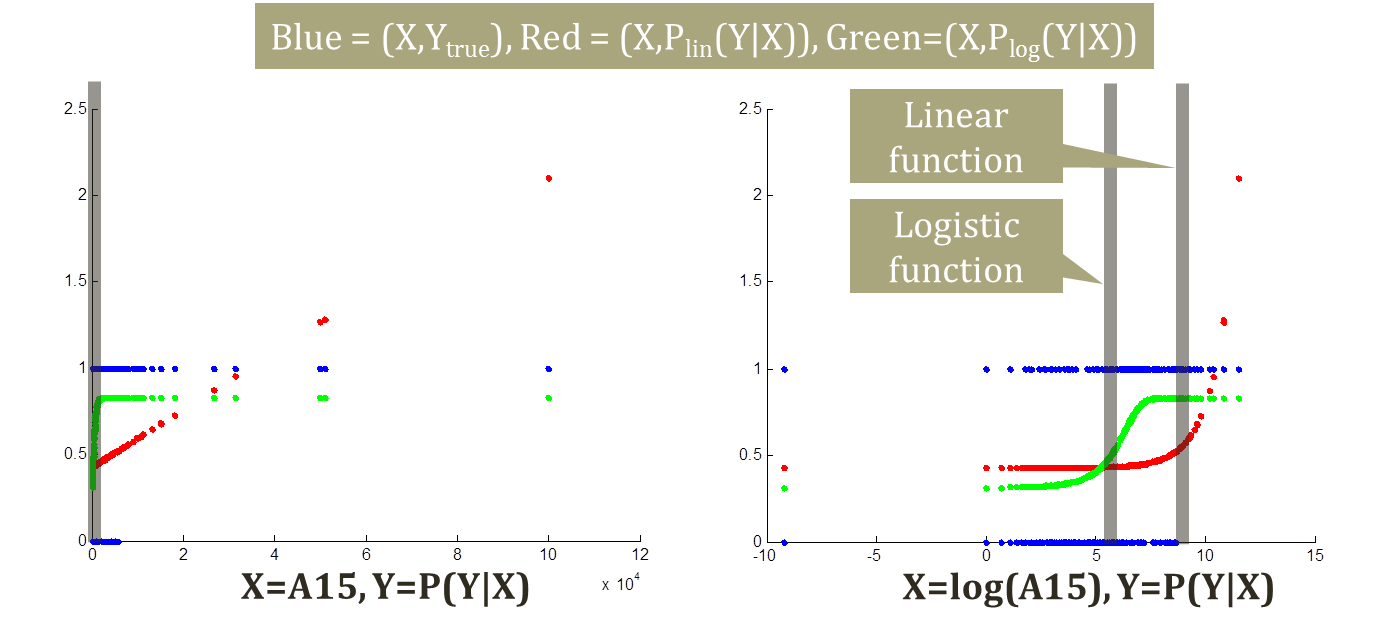
\includegraphics[scale=0.6]{Logistic_Regression_Plot.png}
\caption{x축을 A15, log(A15)로 표현하였을 때 선형회귀와 로지스틱 회귀의 결과}
\label{Figure 4-5}
\end{figure}

%슬라이드 8
\subsection{로지스틱 함수(Logistic Function)}
아까부터 계속 S자형 곡선, 로지스틱 함수 등의 용어를 사용했는데, 이들의 정의를 좀 더 명확히 하고 넘어갈 필요가 있다. 우선, Sigmoid 함수의 정의부터 살펴보자.
\begin{itemize}\itemsep0pt
\item 실수 집합에서 정의된 함수 $f: \mathds{R} \to \mathds{R}$가 다음의 조건을 만족할 때, Sigmoid 함수라고 부른다;
\subitem 1) $f$는 유계(Bounded) 함수, 즉 함수값이 특정 범위 내에 갇혀 있다.
\subitem 2) $f$는 미분가능한 함수이다.
\subitem 3) $f$는 항상 양의 미분계수를 가지는 단조 증가(Monotonically Increasing)함수이다.
\end{itemize}

\indent Sigmoid 함수 중에서 특히, (-1,1)의 개구간에서 함수값이 정의되는 것들을 모아보면 다음의 그림과 같다. Hyperbolic tangent 함수와 Arc tangent 함수도 Sigmoid 함수임을 확인하자. (이 두 함수는 나중에 신경망(Neural Network)을 공부할 때 자주 나오는 함수들이다.)
\begin{figure}[ht]
\centering
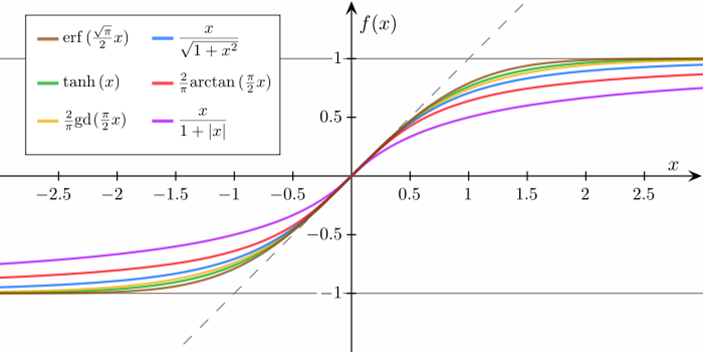
\includegraphics[scale=0.8]{Sigmoid_Functions.png}
\caption{다양한 종류의 Sigmoid 함수들}
\label{Figure 4-6}
\end{figure}

\indent 우리는 특히 지수함수의 역수 형태인 로지스틱 함수를 다음과 같이 정의할 것이다;
\begin{equation*}f(x) = \frac{1}{1+e^{-x}} \tag{4-1}\end{equation*} 이와 같이 정의하였을 때, 이 함수는 개구간 (0,1)에서 함수값을 갖는 Sigmoid 함수이다. 이 함수는 1844년 인구 성장 모델(Population Growth Model)을 연구하던 과학자 Pierre Francois Verhulst 에 의해 처음 사용되었으며, 이름 또한 피에르가 직접 명명하였다.  로지스틱 함수는 앞으로 배울 신경망뿐만 아니라 생태학, 생물수학, 화학, 경제학, 지구과학, 수리심리학, 사회학, 정치학, 언어학 등 수많은 분야에서 사용되고 있다. 그리고 이 함수의 역함수인 다음을 로짓(Logit) 함수라 부른다. \begin{equation*}f^{-1}(x) = log(\frac{x}{1-x}) \tag{4-2}\end{equation*}
\begin{figure}[ht]
\centering
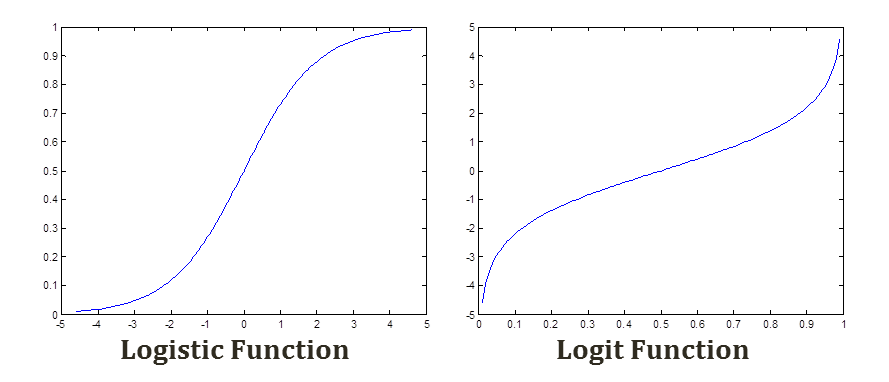
\includegraphics[scale=0.7]{Logistic_Functions.png}
\caption{로지스틱 함수와 로짓 함수}
\label{Figure 4-7}
\end{figure}

\indent 로지스틱 함수의 최대 장점은 무한번 미분가능하면서도, 미분하기가 아주 쉽다는 것인데,  이는 로지스틱 회귀를 이용한 최적화 과정에서 미분값을 0으로 두고 방정식을 푸는 방법을 아주 쉽게 적용할 수 있음을 의미한다. 

%슬라이드 9
\subsubsection{로지스틱 함수를 이용한 Fitting}
로지스틱 함수를 Fitting 하기 위하여, 로짓(Logit)함수로부터 시작하자. 이는 로지스틱 함수의 역함수이므로 정의역은 0과 1 사이에서 정의된다. 즉, x값을 일종의 확률로 생각할 수 있게 된다. 따라서 로그 안의 x 부분을 모두 확률의 $p$로 바꾸고, $f(x)$ 자리에는 (역함수의 함수값이므로) 본래 데이터인 x를 대입할 수 있다. (식 4-4) 주어진 함수의 사이즈 및 위치를 조절하기 위해 식 4-5 와 같이 좌변을 변형한 후 매트릭스의 곱 형태로 바꾸면 최종 형태인 식 4-6 과 같이 표현할 수 있다.
\begin{align*}
&f(x) = log(\frac{x}{1-x})				\tag{4-3}\\
&\to x=log(\frac{p}{1-p}) 			\tag{4-4}\\
&\to ax+b = log(\frac{p}{1-p})		\tag{4-5}\\
&\to X\theta = log(\frac{p}{1-p})		\tag{4-6}
\end{align*}

\indent 로지스틱 회귀로 넘어가기 전에, 조건부 확률을 왜 선형회귀로 추정하면 안되는지 다시 한 번 상기하자. $P(Y\mid X)$을 근사시킬 때, 선형회귀를 이용한다면 다음과 같은 식이 성립한다; \begin{equation*}X\theta = P(Y\mid X) \tag{4-7}\end{equation*} 하지만, 독립변수의 값에 따라 확률값이 $0 \sim 1$ 사이를 벗어나는 결과를 가져온다. 반면, 로지스틱 회귀는 다음과 같은 식을 만족한다; \begin{equation*}X\theta = log \left( \frac{P(Y\mid X)}{1-P(Y\mid X)} \right) \tag{4-8}\end{equation*}

%슬라이드 10
\subsection{로지스틱 회귀(Logistic Regression)}
로지스틱 회귀란, 이항(Binomial) 또는 다항(Multinomial)적인 결과값을 가지는 확률 변수(Random Variable)의 확률 분포(Probabilistic Distribution)를 추정하는 Classifier 중 하나로써, 특히 로지스틱 함수를 사용하는 것이다. 앞서 말했듯이, 우리는 조건부 확률을 로지스틱 함수에 피팅할 것이다. 로지스틱 회귀의 좀 더 공식적인 정의는 다음과 같다;
\begin{equation*}
P(y \mid x) = \mu(x)^{y}(1-\mu(x))^{1-y}				\tag{4-9}
\end{equation*}
\begin{equation*}
\mu(x) = \frac{1}{1+e^{-\theta^{T}x}} = P(y=1 \mid x)	\tag{4-10}
\end{equation*}
\begin{equation*}
X\theta = log\left(\frac{P(Y \mid X)}{1- P(Y \mid X)}\right) \to P(Y \mid X) = \frac{e^{X\theta}}{1+e^{X\theta}} \tag{4-11}
\end{equation*}

\indent $P(y \mid x)$가 확률 $\mu (x)$인 이항분포를 따른다고 했을 때 식 4-9 와 같은 형태로 표현할 수 있다. 만약 이 $\mu (x)$가 로지스틱 함수의 형태라면 어떨까? 그렇다면 식 4-10 의 형태로 나타나고, 이전에 보았던 식 4-8 을 정리하면 4-11 의 결과를 얻을 수 있다.

%슬라이드 11
\subsubsection{매개변수 \texorpdfstring{$\theta$}{Lg} 값 찾기}
지난 1, 2 단원에서 Maximum Likelihood Estimator(MLE)라는 추정값을 사용했던 것을 상기하자. MLE $\hat{\theta}$은 특정 결과물(데이터셋)을 만들어내는 가장 '그럴듯한' Estimator로서, Likelihood인 $P(D \mid \theta)$를 최대로 만드는 $\theta$값을 의미한다;
\begin{equation*}\hat{\theta} = argmax_{\theta}P(D \mid \theta) \tag{4-12} \end{equation*}

\indent 로지스틱 회귀에서 파라미터 $\theta$를 찾는 과정에서는 단순한 MLE가 아닌 Maximum Conditional Likelihood Estimator(MCLE)를 사용할 것이다. MCLE는 주어진 관측값의 확률을 최대로 하는 것은 같으나, 조건부로 또 다른 관측값이 주어졌다고 가정하게 된다.
\begin{align*}
\hat{\theta} 	&=argmax_{\theta}P(D \mid \theta)												\tag{4-13}\\
			&=argmax_{\theta}\prod_{1\le i\le N}P(Y_{i} \mid X_{i};\theta)					\tag{4-14}\\
			&=argmax_{\theta}log\left(\prod_{1\le i\le N}P(Y_{i} \mid X_{i};\theta)\right)		\tag{4-15}\\
			&=argmax_{\theta}\sum_{1\le i\le N}log(P(Y_{i} \mid X_{i};\theta))				\tag{4-16}
\end{align*}

\indent 식 4-14 의 $N$은 주어진 전체 데이터의 크기를 의미하며, 이 때의 Likelihood는 각각의 사건이 발생할 확률의 곱으로(개별 사건의 독립성을 가정) 표현된다. Argument Maximum은 주어진 식의 값을 최대로 하는 $\theta$를 찾는 것이므로 로그를 취하더라도 그 값은 변하지 않는다. (식 4-15) 최종적으로 MCLE $\hat{\theta}$의 형태는 식 4-16 과 같은 합의 형태로 나타낼 수 있다. 그렇다면 조건부 확률인 $P(Y_{i} \mid X_{i};\theta)$는 어떤 식으로 표현할 수 있을까? 앞서 우리는 조건부 확률이 이항분포를 따른다고 가정하였는데, 마찬가지로 다음과 같이 이항분포를 따른다고 가정할 것이다;
\begin{equation*}P(Y_{i} \mid X_{i};\theta) = \mu(X_{i})^{Y_{i}}(1-\mu(X_{i}))^{1-Y_{i}}\tag{4-17} \end{equation*}
\begin{align*}
log(P(Y_{i} \mid X_{i};\theta))	&=Y_{i}log(\mu(X_{i}))+(1-Y_{i})log(1-\mu(X_{i}))	\tag{4-18}\\
	&=Y_{i}\left\{log(\mu(X_{i}))-log(1-\mu(X_{i}))\right\}+log(1-\mu(X_{i}))			\tag{4-19}\\
	&=Y_{i}log\left(\frac{\mu(X_{i})}{1-\mu(X_{i})}\right)+log(1-\mu(X_{i}))			\tag{4-20}\\
	&=Y_{i}X_{i}\theta+log(1-\mu(X_{i}))											\tag{4-21}\\
	&=Y_{i}X_{i}\theta-log(1+e^{X_{i}\theta})										\tag{4-22}
\end{align*}

\indent 조건부 확률에 로그를 취하여 식을 정리해주면 위의 결과를 얻을 수 있고, (식 4-22) 결론적으로 다음과 같이 정리할 수 있다.

%슬라이드 12
\begin{align*}
\hat{\theta}	&=argmax_{\theta}\sum_{1\le i\le N}log(P(Y_{i} \mid X_{i};\theta)) \tag{4-23}\\
&=argmax_{\theta}\sum_{1\le i\le N}\left\{Y_{i}X_{i}\theta - log(1+e^{X_{i}\theta})\right\}	\tag{4-24}
\end{align*}

\indent 이전에 로지스틱 함수의 장점을 설명했던 부분을 상기하자. 이 함수는 무한번 미분가능(infinitely differentiable)하고, 계산하기가 비교적 편리하므로 최적화(Optimization) 과정에서 미분계수가 0이라고 놓고 방정식의 해를 구할 것이다. 단, 여기서는 $\theta$의 Component인 $\theta_{j}$에 대해 각각 편미분을 하여, Component별로 미분계수가 0인 지점을 찾는다.
\begin{align*}
\frac{\partial}{\partial \theta_{j}}&\left\{\sum_{1\le i\le N}Y_{i}X_{i}\theta - log(1+e^{X_{i}\theta})\right\} \tag{4-25}\\
&=\left\{\sum_{1\le i\le N}Y_{i}X_{i,j}\right\}+\left\{\sum_{1\le i\le N}-\frac{1}{1+e^X_{i}\theta}\times e^{X_{i}\theta}\times X_{i,j}\right\}								\tag{4-26}\\
&=\sum_{1\le i\le N}X_{i,j}\left(Y_{i}-\frac{e^{X_{i}\theta}}{1+e^{X_{i}\theta}} \right)	\tag{4-27}\\
&=\sum_{1\le i\le N}X_{i,j}(Y_{i}-P(Y_{i}=1 \mid X_{i};\theta)) =0					\tag{4-28}
\end{align*}

\indent 식 4-28 의 결과를 살펴보면, 앞서 나왔던 MLE나 MAP와 같이 $\theta = \cdots$와 같이 닫힌 형태로 나오지 않음을 알 수 있다. 이런 경우에는, 다양한 방법론을 적용하여 해당 방정식을 만족하는 $\theta$ 값을 근사하여 사용해야 한다. 따라서, 다음 챕터에서는 Gradient Descent 라는 근사법에 대해 배워볼 것이다.

%슬라이드 13
\section{Gradient Method}

%슬라이드 14
\subsection{테일러 전개(Taylor Expansion)}
경사법(Gradient Descent Method)을 배우기 위해서는, 먼저 함수의 테일러 전개에 대해 이해해야 한다. 테일러 전개는 영국의 수학자 브룩 테일러(Brook Taylor)에 의해 제안된 것으로, 특정 조건을 만족시키는 함수를 지역적 특성(Local Properties)을 이용하여 근사(Approximation)하는 방법이다. 좀 더 구체적으로 말하면, 한 점에서의 함수값 및 n차 미분계수 값을 이용하여 해당 함수와 비슷한 다항함수를 만드는 것이라 할 수 있겠다. 특히 무한 번 미분가능하고 수렴이 전제된다면 이 함수를 무한급수(Series)의 형태로 나타낼 수 있는데, 이러한 무한급수를 이용한 방법은 계량적인 방법을 이용하는 다양한 분야에서 많이 사용되고 있다. 실생활에서의 예로는 계산기가 무리함수의 값을 구할 때 테일러 근사의 n번째 항까지의 값을 계산하여 나타내므로 우리 생활에 매우 유용하게 이용되고 있다고 말 할 수 있다. \\
\indent 임의의 함수 $f(x)$의 점 $x=a$에서의 테일러 전개는 다음과 같이 표현할 수 있다.
\begin{align*}
f(x)	&=f(a) + \frac{f\prime(a)}{1!}(x-a) + \frac{f\prime \prime (a)}{2!}(x-a)^{2} + \cdots \tag{4-29}\\
	&=\sum_{n=0}^{\infty}\frac{f^{(n)}(a)}{n!}(x-a)^{n} \tag{4-30}
\end{align*}

\indent 함수 $e^{x}$와 $log(x)$에 대하여 각각 $x=a=0$, $x=a=0.5$ 점에 대한 테일러 전개를 해본 후 다음과 비교해보도록 하자. \\
when $a=0$, 
\begin{equation*}
e^{x} = 1+\frac{e^{0}}{1!}(x-0)^{1}+\frac{e^{0}}{2!}(x-0)^{2}+ \cdots \tag{4-31}
\end{equation*}
when $a=0.5$, 
\begin{equation*}
log(x) = log(0.5) + \frac{\frac{1}{0.5}}{1!}(x-0.5)^{1}+\frac{\frac{1}{0.5^{2}}}{2!}(x-0.5)^{2}+\cdots \tag{4-32}
\end{equation*}

\indent 테일러 전개는 무한 번 미분가능한(혹은 Smooth한) 함수에 대하여 실시하는데, 이렇게 매끄러운 함수에 대해서는 경사법(Gradient Descent Method)을 사용할 수 있다.

%슬라이드 15
\subsection{경사법(Gradient Descent/Ascent)}
경사법은 미분가능한 함수 $f(x)$에 대하여, 주어진 위치 $x_{1}$에서 시작해서 이 점을 점점 이동시키며 함수값이 증가 또는 감소하도록 하는 방법이다. 그렇다면 함수값이 변화하는 방향을 어떻게 찾을 것인가? 그리고 얼마나 빠르게 이동시킬 것인가? 두 가지 질문이 자연스레 나오게 되는데, 함수의 Gradient 방향 또는 그 반대 방향을 이용하면 가장 효율적으로 함수값을 변화시킬 수 있으므로 이 방법을 경사법(Gradient Descent/Ascent)이라고 부르는 것이다. 흔히 기계학습에서 이용하는 경사법에서는 점을 이동시키는 속력은 사람이 외부에서 정해주고, 방향은 프로그램이 직접 찾도록 하는 것이 일반적이다. \\
\indent 경사법이 어떤 원리에 의해 작동하는지 이해하기 위하여 다음을 살펴보자.
\begin{equation*}f(x) = f(a) + \frac{f^{\prime}(a)}{1!}+O(\mid x-a \mid^{2}) \tag{4-33} \end{equation*}
\indent 식 4-33은 Big O notation을 이용하여 차수가 2 이상인 항을 모두 묶고, $a=x_{1}$, $x=x_{1}+h\textbf{u}$ 로 둔다. (Big O 표현의 정의는 이 챕터의 마지막에 정리하였다.) 여기서 $\textbf{u}$는 방향벡터를, h는 변하는 속력을 의미한다. 위의 식을 다시 표현하면 다음과 같이 나타낼 수 있다;
\begin{align*}
f(x_{1}+h\textbf{u}) &= f(x_{1}) + hf^{\prime}(x_{1})\textbf{u} + h^{2}O(1) \tag{4-34} \\
f(x_{1}+h\textbf{u}) &- f(x_{1}) = hf^{\prime}(x_{1})\textbf{u} \tag{4-35}
\end{align*}

\indent 식 4-34에서, O notation 안의 식은 $h$의 이차항에 한정(Confined)되어 있는데 이 값은 $h$가 매우 작은 수라면 무시할 수 있으므로, 식 4-35와 같은 근사를 할 수 있다. 그리고 방향벡터인 $\textbf{u}$는 경사법의 정의에서 설명했듯이, 이 함수의 경사(Gradient) 방향으로 설정하면 가장 효율적으로 함수값을 증가시키거나 감소시킬 수 있으므로 다음과 같이 쓸 수 있다;
\begin{align*}
\textbf{u}^{\ast} &= argmin_{\textbf{u}}\{f(x_{1}+h\textbf{u})-f(x_{1})\} \tag{4-36} \\
&= argmin_{\textbf{u}}hf^{\prime}(x_{1})\textbf{u} \tag{4-37} \\
&= -\frac{f^{\prime}(x_{1})}{\mid f^{\prime}(x_{1}) \mid} \tag{4-38}
\end{align*}

\indent 여기서는 함수의 경사 방향과 반대로(Argument Minimum 사용 혹은 마지막의 음의 부호로부터 알 수 있듯이) 설정하였으므로, Gradient Descent 방법이라 할 수 있겠다. 좀 더 설명하자면, Argument Minimum 괄호 안의 식 $f(x_{1}+h\textbf{u})-f(x_{1})$이 최소화되려면 해당 값이 음수, 즉 $f(x_{1}+h\textbf{u}) \leq f(x_{1})$ 이 성립해야 한다. 따라서 함수값이 감소하는 방향인 것을 알 수 있고, 그 중에서도 특히 경사방향과 정반대(180도), 혹은 음의 방향으로 이동한다면 가장 효율적으로 함수값을 감소시킬 수 있다는 것이다. \\
\indent 따라서 다음 점의 좌표 $x_{t+1}$를 다음과 같이 업데이트 시켜야 한다;
\begin{align*}
x_{t+1} \gets x_{t} + h\textbf{u}^{\ast} = x_{t} - h\frac{f^{\prime}(x_{1})}{\mid f^{\prime}(x_{1}) \mid} \tag{4-39}
\end{align*}

\indent 다시 우리의 본래 목적으로 돌아오도록 하자. 우리는 MCLE를 찾기 위해, 다음의 조건을 만족시키는 매개변수 $\theta$의 값을 찾아야 한다; \\
$\hat{\theta}=argmax_{\theta}\sum_{1\le i\le N}log(P(Y_{i} \mid X_{i};\theta))$ (식 4-23) 경사법을 적용하기 위하여, 함수 $f(\theta)$를 $f(\theta) = \sum_{1\leq i \leq N}log(P(Y_{i} \mid X_{i}; \theta))$와 같이 정의하자. 최초 매개변수 $\theta_{1}$값을 임의로 설정하고, 이 점의 좌표를 서서히 움직이면서 함수 $f(\theta)$의 값이 증가하도록 만드는데, 이 때는 Gradient Ascent 를 이용하여 경사 방향으로 움직이도록 설정하면 된다. 

%슬라이드 16
\subsubsection{Gradient Descent 의 작동 원리 예시}
다음의 로젠브룩(Rosenbrock) 함수를 살펴보자. 
\begin{equation*} f(x_{1}, x_{2}) = (1 - x_{1})^{2} + 100(x_{2} - x_{1}^{2})^{2} \tag{4-40}\end{equation*}
\begin{figure}[ht]
\centering
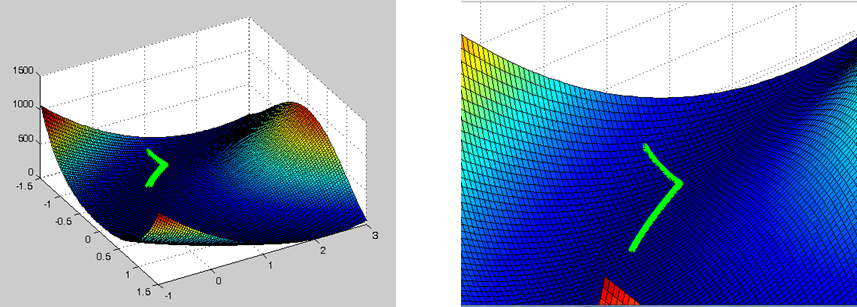
\includegraphics[scale=0.8]{Rosenbrock_function.png}
\caption{로젠브룩 함수의 그래프}
\label{Figure 4-8}
\end{figure}

\indent 먼저 함수의 형태로부터, 각각의 항이 0일 때 Global Minimum을 가지는 것을 알 수 있으므로, 좌표 (1,1)에서 최소값을 갖는다. (혹은 편미분계수가 0이 되는 지점을 찾는다.) 이 예제의 경우에는 이렇게 극점의 위치를 쉽게 구할 수 있었지만, 만약 함수의 형태가 복잡하거나, 미분계수가 0이 되는 지점의 연립방정식이 닫힌 형태(Closed Form)의 해를 가지지 않는다면 어떻게 할 것인가?
\indent 시작점의 위치 \textbf{$x^{0}$}가 (-1.3, 0.9)라고 가정하자. Gradient Descent 방법을 이용하기 위하여 우선 경사(Gradient) 방향을 알아내야 한다.
\begin{align*}
&\frac{\partial}{\partial x_{1}}f(x_{1},x_{2}) = -2(1-x_{1})-400x_{1}(x_{2}-x_{1}^{2})^{2} \tag{4-41}\\
&\frac{\partial}{\partial x_{2}}f(x_{1},x_{2}) = 200(x_{2}-x_{1}^{2})^{2} \tag{4-42}
\end{align*}

\indent \textbf{$x^{0}$}의 좌표를 대입하여 계산하면,
\begin{align*}
\textbf{$f^{\prime}(x^{0})$}
&= \left( \frac{\partial}{\partial x_{1}}f(x_{1},x_{2}), \frac{\partial}{\partial x_{2}}f(x_{1},x_{2}) \right) \tag{4-43} \\
&= (-415.4, -158) \tag{4-44}
\end{align*}

\indent 시작점인 \textbf{$x^{0}$}를 이동시키는 속력은 $h=0.001$로 정하였다. 함수값이 감소하는 방향으로 이동시키는 Gradient Descent를 사용할 것이므로 \textbf{$x^{0}$}에서 $h\frac{f^{\prime}(x_{0})}{\mid f^{\prime}(x_{0}) \mid}$ 만큼을 빼줘야 할 것이다.
\begin{align*}
\textbf{$x^{1}$} & \gets \textbf{$x^{0}$} - h\frac{f^{\prime}(x_{0})}{\mid f^{\prime}(x_{0}) \mid} \tag{4-45} \\
\textbf{$x^{1}$} & = (-1.3 - 0.001 \times -415.4/444.4335, 0.9 - 0.001 \times -158/444.4335 ) \tag{4-46} \\
& = (-1.2991, 0.9004) \tag{4-47}
\end{align*}

\indent 위의 과정을 충분히 많이 수행하면 Global Minimum으로 서서히 수렴할 것이다.
\begin{figure}[ht]
\centering
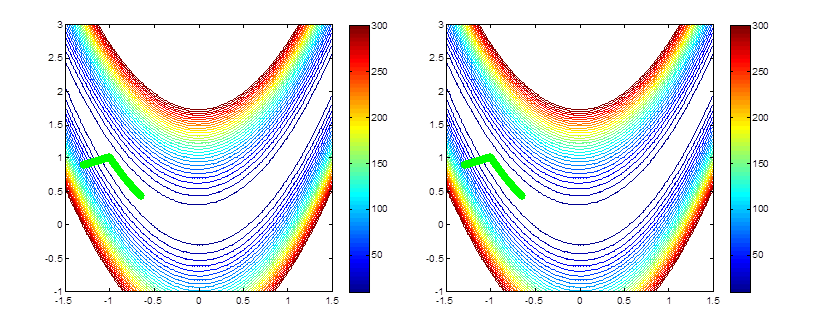
\includegraphics[scale=0.9]{GD_Rosenbrock.png}
\caption{Gradient Descent 결과 점의 이동 경로}
\label{Figure 4-9}
\end{figure}

%슬라이드 17
\subsection{Gradient Ascent를 이용하여 \texorpdfstring{$\theta$}{Lg}값 찾기}
우리는 이 단원의 앞 부분에서 MCLE를 구하는 과정중 다음과 같은 중간 결과들을 얻을 수 있었다. ($f(\theta)$는 Likelihood이므로, 이를 최대화시켜야 함) 식 4-23 과 4-28 을 참고하자.
\begin{itemize}
\item $\hat{\theta} = argmax_{\theta}\sum_{1 \leq i \leq N}log(P(Y_{i} \mid X_{i}; \theta))$
\item $f(\theta) = \sum_{1 \leq i \leq N}log(P(Y_{i} \mid X_{i}; \theta))$
\item $\frac{\partial f(\theta)}{\partial \theta_{j}} = \frac{\partial}{\partial \theta_{j}}\{ \sum_{1 \leq i \leq N}log(P(Y_{i} \mid X_{i}; \theta)) \}$
\item[] $= \sum_{1 \leq i \leq N}X_{i, j}(Y_{i} - P(y=1 \mid x; \theta))$
\end{itemize}

\indent 우리가 찾고자 하는 $\hat{\theta}$은 Argument Maximum으로 함수 $f(\theta)$의 값이 최대가 되는 지점을 찾는 것이므로 여기서는 Gradient Ascent를 이용하면 된다. 따라서, $x_{t+1}$를 $x_{t}\textbf{+}h\dfrac{f^{\prime}(x_{t})}{\mid f^{\prime}(x_{t}) \mid}$로 업데이트 시켜줘야 한다.
\begin{equation*}
x_{t+1} \gets x_{t} + h\textbf{$u^{\ast}$} = x_{t} + h\frac{f^{\prime}(x_{t})}{\mid f^{\prime}(x_{t}) \mid} \tag{4-48}
\end{equation*}

\indent 따라서, 매개변수 \textbf{$\theta$}를 반복적으로 업데이트 시켜주기 위해서는 다음과 같이 진행하여야 한다;
\begin{align*}
\theta_{j}^{t+1} \gets & \theta_{j}^{t} + h\frac{\partial f(\theta^{t})}{\partial \theta_{j}^{t}} \tag{4-49}\\
= &\theta_{j}^{t} + h\left\{ \sum_{1 \leq i \leq N}X_{i, j}(Y_{i}-P(Y=1 \mid X_{i}; \theta^{t})) \right\} \tag{4-50} \\
= &\theta_{j}^{t} + \frac{h}{C}\left \{ \sum_{1 \leq i \leq N}X_{i, j}\left(Y_{i}-\frac{e^{X_{i}\theta^{t}}}{1+e^{X_{i}\theta^{t}}}\right) \right \} \tag{4-51}
\end{align*}

\indent 여기서 상수 $C$는 중괄호 안의 벡터의 크기로, 이렇게 나눠줌으로써 보정되는 부분을 속력($h$)과 방향벡터의 곱으로 나타낼 수 있게 된다. 시작위치인 $\theta_{j}^{0}$는 임의로 설정하면 된다. \\
\indent 드디어, 로지스틱 회귀의 결과인 $\hat{\theta}$를 구하는 방법을 완성하였다! 경사법을 시작하기 전 부분에서 언급하였듯이, 로지스틱 회귀를 이용하여 구해야 하는 매개변수의 최적값 $\hat{\theta}$는 닫힌 형태의 꼴로 나오지 않으므로, Gradient Descent/Ascent 등의 방법을 이용하여 Numerical 한 접근을 해야했다. 다음으로는 이를 매트랩 상에서 구현해보는 예제를 살펴보자.

%슬라이드 18
\subsubsection{Matlab Exercise}
생략

%슬라이드 19
\subsection{Linear Regression Revisited}
여기까지 로지스틱 회귀와, 그 결과 매개변수의 최적값인 $\hat{\theta}$를 구하기 위해 경사법을 이용하는 것까지 살펴보았다. 이렇게 할 수밖에 없었던 이유는 $\hat{\theta}$를 구하는 식의 형태가 깔끔하게 닫힌 형태로 나오지 않았기 때문이다. 반면, 선형 회귀의 경우 지난 1,2 단원에서 살펴보았듯이 아주 깔끔한 형태로 해를 구할 수 있었다.
\begin{align*}
\hat{\theta} &= argmin_{\theta}(f-\hat{f})^{2} \tag{4-52} \\
&= argmin_{\theta}(Y-X\theta)^{2} \tag{4-53} \\
&= argmin_{\theta}(Y-X\theta)^{T}(Y-X\theta) \tag{4-54} \\
&= argmin_{\theta}(\theta^{T}X^{T}X\theta - 2\theta^{T}X^{T}Y + Y^{T}Y) \tag{4-55} \\
&= argmin_{\theta}(\theta^{T}X^{T}X\theta - 2\theta^{T}X^{T}Y) \tag{4-56} \\
&\to \nabla_{\theta}(\theta^{T}X^{T}X\theta - 2\theta^{T}X^{T}Y) = 0 \tag{4-57} \\
&\to 2X^{T}X\theta - 2X^{T}Y = 0 \tag{4-58} \\
\therefore \; &\theta = (X^{T}X)^{-1}X^{T}Y \tag{4-59}
\end{align*}

\indent 하지만, 닫힌 형태의 해를 구할 수 있는 공식이 있음에도 이를 이용하기가 쉽지 않을 때가 있다. 바로 데이터의 사이즈인 행렬 $X$의 크기가 아주 클 때이다. 가장 흔히 사용되는 역행렬을 구하는 방법인 Gaussian-Elimination Algorithm은 $X$가 $n \times n$ 사이즈일 때, Computational Complexity 가 $n^{3}$의 속도로 증가하고, 이에 비해 훨씬 효율적인 Optimized CW-like Algorithm을 이용한다고 하더라도 Complexity는 $n^{2.373}$의 속도로 증가한다. 따라서 우리가 구성한 데이터 셋의 Feature의 갯수(Attribute의 갯수)가 많으면 많을수록 역행렬을 구하는 데에 걸리는 시간은 엄청나게 증가한다. 이러한 상황을 피하기 위해, 선형회귀 문제에서도 경사법을 이용할 수 있다. \\
\indent 선형회귀는 목표함수와 근사함수 사이의 차이의 제곱을 최소화하는 방법으로 풀었던 것을 상기하자. 이것을 수식으로 표현하면 다음과 같다.
\begin{align*}
\hat{\theta} &= argmin_{\theta}(f-\hat{f})^{2} \tag{4-60} \\
&= argmin_{\theta} (Y-X\theta) \tag{4-61} \\
&= argmin_{\theta} \sum_{1 \leq i \leq N}(Y^{i} - \sum_{1 \leq j \leq d}X_{j}^{i}\theta_{j})^{2} \tag{4-62}
\end{align*}

\indent 여기서는 오차를 최소화하는 것이 목적이므로 Argument Minimum이 사용되었고, argmin 안 부분의 함수값을 점점 감소시키는 방향으로 경사법(Gradient Descent)을 이용하면 될 것이다. 따라서 다음과 같이 진행한다.
\begin{align*}
\to &\frac{\partial}{\partial \theta_{k}}\sum_{1 \leq i \leq N}(Y^{i}-\sum_{1 \leq j \leq d}X_{j}^{i}\theta_{j})^{2} \tag{4-63} \\
&= -\sum{1 \leq i \leq N}2(Y^{i}-\sum_{1 \leq j \leq d}X_{j}^{i}\theta_{j})X_{k}^{i} \tag{4-64}
\end{align*}
\begin{align*}
\therefore \: \theta_{k}^{t+1} &\gets \theta_{k}^{t}-h\frac{\partial f(\theta^{t})}{\partial \theta_{k}^{t}} \tag{4-65} \\
&= \theta_{k}^{t}+h\sum_{1 \leq i \leq N}2(Y^{i}-\sum_{1 \leq j \leq d}X_{j}^{i}\theta_{j})X_{k}^{i} \tag{4-66}
\end{align*}

\indent 이것으로, 로지스틱 회귀에서 열린 형태의 식이 나오는 매개변수의 최적값을 순차적으로 학습하는 방법 및 데이터의 사이즈가 매우 커서 닫힌 형태의 공식을 사용하기 힘든 경우의 선형 회귀에 대해 매개변수를 학습하는 방법에 대해 배워보았다. 그렇다면 앞 단원에서의 Naive Bayes 방법과 로지스틱 회귀 방법에는 어떤 차이가 있을까? 이에 대해 다음 장에서 살펴보자.

%슬라이드 20
\section{Naive Bayes VS Logistic Regression}
이 장에서는 지난 단원에서 배웠던 Naive Bayes Classifier 와 로지스틱 회귀를 비교해 보고자 한다. 하지만, 이번 단원에서 로지스틱 회귀는 신용평가 데이터의 연속적인 항목에 대해서만 분석해보았다. 이는 이전 단원에서 NB Classifier를 다룰 때 이산적인 데이터를 사용했던 것과 대치된다. 따라서 NB Classifier 함수를 연속적인 확률변수에 대해서 다룰 수 있도록 일반화할 필요가 있다.

%슬라이드 21
\subsection{Gaussian Naive Bayes}
이산적인(Discrete) 데이터만 다루었던 Naive Bayes Classifier를 연속적인(Continuous) 경우에도 사용할 수 있도록 정규분포(Gaussian Distribution)를 이용하여 Gaussian Naive Bayes Classifier 를 정의하자. 먼저, 지난 단원에서 NB Classifier는 다음과 같이 정의하였다;
\begin{equation}
f_{NB}(x) = argmax_{Y=y}P(Y=y)\prod_{1 \leq i \leq d}P(X_{i} = x_{i} \mid Y=y) \tag{4-67}
\end{equation}

\indent 여기서 $P(Y=y)$는 확률변수 $Y$에 대해 가지고 있는 사전 정보, $P(X_{i} = x_{i} \mid Y=y)$는 $Y$가 주어졌을 때의 조건부 확률(Class Conditional Density)이었다. $d$는 데이터 $X$의 Input Feature의 갯수에 해당한다. 그리고 개별 Attibute에 대해 독립성을 가정하여 곱의 형태로 표현했던 것이 NB 가정의 핵심이었다.
\begin{align}
&P(X_{i} \mid Y, \mu, \sigma^{2}) = \frac{1}{\sigma \sqrt{2 \pi}}e^{-\frac{(X_{i}-\mu)^{2}}{2 \sigma^{2}}} \tag{4-68} \\
&P(Y=y) = \pi_{1} \tag{4-69}
\end{align}
 
\indent Gaussian NB는 NB Classifier의 표현(식 4-67)에서 마지막 항인 조건부 확률 $P(X_{i} = x_{i} \mid Y=y)$가 정규분포를 따른다고 가정하는데, 평균과 분산이 각각 $\mu$, $\sigma^{2}$인 정규분포의 형태는 식 4-68 과 같이 나타난다. 표기의 편의를 위해 식 4-69 를 가정하자. 마지막으로 4-67 에 4-68, 69 를 대입하면 다음과 같이 표현된다;
\begin{equation}
P(Y)\prod_{1 \leq i \leq d}P(X_{i} \mid Y) = \pi_{k}\prod_{1 \leq i \leq d}\frac{1}{\sigma_{k}^{i}C}exp\left( -\frac{1}{2}\left(\frac{X_{i}-\mu_{k}^{i}}{\sigma_{k}^{i}}\right)^{2} \right) \tag{4-70}
\end{equation}

%슬라이드 22, 23
\subsection{Derivation to Logistic Regression}
조건부 확률 $P(Y \mid X)$를 구할 때, 로지스틱 회귀에서는 변형 없이 그대로 사후 확률(Posterior Probability)의 매개변수를 학습하려 했던 반면, NB에서는 베이즈 정리를 이용하여 사전 확률(Prior Probability)과 조건부 확률(Conditional Probability)의 곱으로 바꿔준 뒤, 바뀐 식의 매개변수를 학습하는 과정이었던 것을 상기하자. 이러한 경우 전자를 Discriminative Classifier, 후자를 Generative Classifier라고 부른다.
\begin{align}
P(Y=y \mid X) &= \dfrac{P(X \mid Y=y)P(Y=y)}{P(X)} \tag{4-71}\\
&=\dfrac{P(X \mid Y=y)P(Y=y)}{P(X \mid Y=y)P(Y=y) + P(X \mid Y=n)P(Y=n)} \tag{4-72}\\
&=\dfrac{P(Y=y)\prod_{1 \leq i \leq d}P(X_{i} \mid Y=y)}{P(Y=y)\prod_{1 \leq i \leq d}P(X_{i} \mid Y=y) + P(Y=n)\prod_{1 \leq i \leq d}P(X_{i} \mid Y=n)} \tag{4-73}
\end{align}

\indent 식 4-71 에서 분모의 $P(X)$는 The Law of Total Expectation 을 이용하여 4-72 와 같이 전개할 수 있다. 여기서 확률변수 $Y$는 Class Variable(이산적)로 오직 두 가지 값만을 가지기 때문에 $P(X)$는 두 개의 항의 합으로 나타난다. (반면, $X$는 연속적) 마찬가지로 Naive Bayes의 가정을 이용하면 식 4-73 과 같이 조건부 확률 $P(X_{i} \mid Y=y)$를 각각의 Attribute에 대한 조건부 확률의 곱으로 표현할 수 있다. 이제 Gaussian NB의 가정, 즉 정규분포 가정을 추가로 설정하여 조건부 확률에 정규분포의 PDF 함수를 대입하도록 하자;
\begin{align}
&P(Y=y\mid X) \notag \\
&=\dfrac{\pi_{1}\prod_{1 \leq i \leq d}\frac{1}{\sigma_{1}^{i}C}exp\left(-\frac{1}{2}\left(\frac{X_{i}-\mu_{1}^{i}}{\sigma_{1}^{i}} \right)^{2} \right)}{\pi_{1}\prod_{1 \leq i \leq d}\frac{1}{\sigma_{1}^{i}C}exp\left(-\frac{1}{2}\left(\frac{X_{i}-\mu_{1}^{i}}{\sigma_{1}^{i}} \right)^{2} \right) + \pi_{2}\prod_{1 \leq i \leq d}\frac{1}{\sigma_{2}^{i}C}exp\left(-\frac{1}{2}\left(\frac{X_{i}-\mu_{2}^{i}}{\sigma_{2}^{i}} \right)^{2} \right)} \tag{4-74}\\
&=\dfrac{1}{1+\dfrac{\pi_{2}\prod_{1 \leq i \leq d}\frac{1}{\sigma_{2}^{i}C}exp\left(-\frac{1}{2}\left(\frac{X_{i}-\mu_{2}^{i}}{\sigma_{2}^{i}} \right)^{2} \right)}{\pi_{1}\prod_{1 \leq i \leq d}\frac{1}{\sigma_{1}^{i}C}exp\left(-\frac{1}{2}\left(\frac{X_{i}-\mu_{1}^{i}}{\sigma_{1}^{i}} \right)^{2} \right)}}\tag{4-75}
\end{align}

\indent 독자들은 위의 과정이 단순히 식을 정리하는 것에 지나지 않는다는 것을 알 수 있을 것이다. 여기서 추가적으로 $Y=y('Yes')$, $Y=n('No')$ 두 가지 Class 값에 대해 주어진 분포가 같은 분산값을 가진다고 가정할 것이다. 즉, $\sigma_{1}^{i} = \sigma_{2}^{i}$ 를 가정한다는 것이다. 그러면 위의 식을 다음과 같이 정리할 수 있다;
\begin{align}
&P(Y=y\mid X) \notag \\
&=\dfrac{1}{1+\dfrac{\pi_{2}\prod_{1 \leq i \leq d}exp\left(-\frac{1}{2}\left(\frac{X_{i}-\mu_{2}^{i}}{\sigma_{2}^{i}} \right)^{2} \right)}{\pi_{1}\prod_{1 \leq i \leq d}exp\left(-\frac{1}{2}\left(\frac{X_{i}-\mu_{1}^{i}}{\sigma_{1}^{i}} \right)^{2} \right)}} \tag{4-76}\\
&=\dfrac{1}{1+\dfrac{\pi_{2}exp\left[-\sum_{1 \leq i \leq d}\left\{\frac{1}{2}\left(\frac{X_{i}-\mu_{2}^{i}}{\sigma_{2}^{i}} \right)^{2} \right\} \right]}{\pi_{1}exp\left[-\sum_{1 \leq i \leq d}\left\{\frac{1}{2}\left(\frac{X_{i}-\mu_{1}^{i}}{\sigma_{1}^{i}} \right)^{2} \right\} \right]}}	 \tag{4-77}\\
&=\dfrac{1}{1+\dfrac{exp\left[-\sum_{1 \leq i \leq d}\left\{\frac{1}{2}\left(\frac{X_{i}-\mu_{2}^{i}}{\sigma_{2}^{i}} \right)^{2} \right\}+log \pi_{2} \right]}{exp\left[-\sum_{1 \leq i \leq d}\left\{\frac{1}{2}\left(\frac{X_{i}-\mu_{1}^{i}}{\sigma_{1}^{i}} \right)^{2} \right\}+log \pi_{1} \right]}} \tag{4-78}\\
&=\dfrac{1}{1+exp\left[-\sum_{1 \leq i \leq d}\left\{\frac{1}{2}\left(\frac{X_{i}-\mu_{2}^{i}}{\sigma_{2}^{i}} \right)^{2} \right\}+log \pi_{2}+\sum_{1 \leq i \leq d}\left\{\frac{1}{2}\left(\frac{X_{i}-\mu_{1}^{i}}{\sigma_{1}^{i}} \right)^{2} \right\} -log \pi_{1} \right]} \tag{4-79}
\end{align}
\begin{align}
&=\dfrac{1}{1+exp\left[\sum_{1 \leq i \leq d}-\frac{1}{2(\sigma_{1}^{i})^{2}}\left\{ (X_{i}-\mu_{1}^{i})^{2} -(X_{i}-\mu_{2}^{i})^{2}\right\}+log \pi_{2}-log \pi_{1} \right]} \tag{4-80}\\
&=\dfrac{1}{1+exp\left[\sum_{1 \leq i \leq d}-\frac{1}{2(\sigma_{1}^{i})^{2}}\left\{2(\mu_{2}^{i}-\mu_{1}^{i})X_{i} + (\mu_{1}^{i})^{2} - (\mu_{2}^{i})^{2}) \right\}+log \pi_{2}-log \pi_{1} \right]} \tag{4-81}
\end{align}

\indent 위 결과를 식 4-11 과 비교해보자. 식의 형태가 근본적으로 같다는 것을 알 수 있을 것이다. 특히, Exponential 괄호 안의 부분을 살펴보면, $X_{i}$에 관한 일차식인 것을 확인할 수 있는데, 이는 다시 표현하면 \textbf{$X\theta$}와 같은 형태로 나타낼 수 있다. 즉, 특정 조건을 만족하는 Gaussian Naive Bayes는 근본적으로 Logistic Regression과 같다는 것이다.

%슬라이드 24
\subsubsection{Naive Bayes VS Logistic Regression}
\begin{equation}
P(Y \mid X) = \frac{1}{1+exp\left( -\frac{1}{2(\sigma_{1}^{i})^{2}}\sum_{1 \leq i \leq d}\left\{ 2(\mu_{2}^{i} - \mu_{1}^{i})X_{i}+(\mu_{1}^{i})^{2} - (\mu_{2}^{i})^{2} \right\} +log\pi_{2} - log\pi_{1} \right)} \tag{4-81}
\end{equation}
\indent 앞의 유도과정에서 했던 여러 가지 가정들을 정리해보자; (1) $Y$가 2가지의 이산적인 값을 갖는다는 베르누이 분포 가정, (2) 조건부 확률이 개별 Attribute에 대한 조건부 확률의 곱으로 표현된다는 Naive Bayes 가정, (3) NB가 Gaussian(정규분포) Naive Bayes를 따른다는 가정, (4) 두 가지 Class 값에 대해 같은 분산값을 가진다는 가정 등을 설정하였다. 그 결과, 조건부 확률 $P(Y \mid X)$를 식 4-81 과 같이 나타낼 수 있음을 보였다. 이것은 근본적으로 로지스틱 회귀와 같은 형태의 식인데, 그렇다면 Gaussian NB와 로지스틱 회귀에는 어떤 차이점이 있는 것일까?\\
\begin{equation}
P(Y \mid X) = \frac{1}{1+e^{-\theta^{T}x}} \tag{4-82}
\end{equation}
\indent 	추정해야 하는 매개변수의 갯수 관점에서 이들을 살펴보자. Gaussian NB의 경우, 각 Class의 각 Attribute에 대해 평균과 분산을 알아야 하므로 $4*d$개, 여기에 $\pi_{1}$ 또는 $\pi_{2}$를 알아내야 하므로 총 $4d+1$개의 매개변수를 추정해야 한다. 반면, 로지스틱 회귀에서는 개별 Attribute Feature 와 바이어스 항까지 총 $d+1$개의 매개변수를 추정해야 한다. 그렇다면 추정할 변수의 갯수가 적은 로지스틱 회귀가 더 효율적인 방법이라고 할 수 있을 것이다. 그리고 학계에서도 로지스틱 회귀가 Gaussian NB에 비해 더 좋은 성능을 낸다는 것이 알려져 있다. \\
\indent 하지만 반드시 로지스틱 회귀가 Gaussian NB에 비해 월등한 것은 아니다. 만약 주어진 문제 상황에서 사전 확률(Prior Probability)에 대한 정보가 있어서 이를 응용할 수 있다면, NB Classifier를 이용하는 것이 더 유리할 수 있다.

%슬라이드 25
\subsection{Generative-Discriminative Pair}
앞에서 언급했듯이, Generative Model은 베이즈 정리에 의해 사후 확률(Posterior Probability) $P(Y \mid X)$를 사전 확률(Prior Probability) $P(Y)$와 조건부 확률(Conditional Probability) $P(X \mid Y)$의 곱으로 나타내어 푸는 모델이다. 따라서 사후 확률이 아닌 사전 확률과 조건부 확률의 매개변수들을 추정하게 된다. \\
\indent 반면 Discriminative Model은 사후 확률의 매개변수를 바로 추정하여 푸는 모델이다. 조건부 확률 형태인 사후 확률을 바로 푸는 방법이므로, 조건부 확률을 모델링할 때 사용된다. Generative-Discriminative Pair에 관한 좀 더 깊이 있는 논의는 Ng \& Jordan(2002) 의 논문에서 살펴보길 권한다.

%슬라이드 26
\section*{Acknowledgement}
This slideset is greatly influenced by
\begin{itemize}\itemsep0pt
\item Professor Carlos Guestrin at CMU
\item Professor Eric Xing at CMU
\item Professor Tom Mitchell at CMU
\end{itemize}

%슬라이드 27
\section*{Further Readings}
\begin{itemize}\itemsep0pt
\item Bishop Chapter 4.3, 5.2.1 $\sim$ 5.2.4 \end{itemize}

%보충설명 APPENDIX
\section*{Appendix}
\subsection*{Big O Notation}
실수 집합에서 정의된 두 함수 $f,g$에 대하여, 다음의 두 Statement는 동치이다;
\begin{itemize}\setlength\itemsep{-\parsep}
\item $f(x)=O\left(g(x)\right)$ as $x \to \infty$ \: if and only if
\item $\exists M>0, \exists x_{0}$ such that $\mid f(x)\mid \leq M\mid g(x)\mid$ for all $x\geq x_{0}$
\end{itemize}

\indent 두 번째 표현은 정의역이 특정 범위($x_{0}$보다 큰)를 벗어났을 때, 함수 $f(x)$의 값이 함수 $g(x)$ 값의 상수($M$)배 내에서 움직이도록 한정(Confined)시킬 수 있다는 것이다. 따라서, $f(x)=O\left(g(x)\right)$ 표현은 함수 $f(x)$가 함수 $g(x)$의 최대 상수배 안으로 가둘 수 있다는 것을 의미한다. 다음의 예시를 살펴보자.
\begin{align*}
\mid 6x^{4} - 2x^{3} + 5\mid &\leq 6x^{4} + \mid 2x^{3}\mid + 5 \tag{4-A-1}\\
&\leq 6x^{4} + 2x^{4} + 5x^{4} \tag{4-A-2}\\
&=13x^{4} \tag{4-A-3}\\
\therefore \; \mid 6x^{4} - 2x^{3} + 5\mid &\leq 13x^{4} \tag{4-A-4}
\end{align*}

\indent $x$의 값이 발산하는 경우 이외에도, 특정 값($a$)에 수렴할 때 동일한 표현을 사용할 수 있다. 이 때의 정의는 다음과 같다;
\begin{itemize}\setlength\itemsep{-\parsep}
\item $f(x)=O\left(g(x)\right)$ as $x \to a$ \: if and only if
\item $\exists \delta>0, \exists M>0$, such that $\mid f(x)\mid \leq M\mid g(x)\mid$ when $0<\mid x-a \mid < \delta$
\end{itemize}
\end{document}
%--------------------------------------------------------------------------------------------------
%알고리즘(pseudo-code) 넣기
\indent\rule{10cm}{0.4pt} \\
\begin{algorithm}[H]
	\SetAlgoLined
	\KwData{Training Dataset}
	\KwResult{Find the Correct Hypothesis}
	Initialize $h = h_{0}$
	\For{instance $x$ in $D$}{
		\eIf{$x$ is positive}{
			\For{Feature $f$ in $O$}{
				\eIf{$f_{i}$ in $h == f_{i}$ in $x$}{
					Do Nothing;
				}{
					$f_{i}$ in $h = f_{i}$ in $h \cup f_{i}$ in $x$
				}
			}
		}{}
	}
\end{algorithm}

\indent \rule{10cm}{0.4pt} \\
%--------------------------------------------------------------------------------------------------
%아이템 간격조절해서 넣기
\begin{itemize}\setlength\itemsep{-\parsep}
	\item Instances
	\begin{description}\setlength\itemsep{-\parsep}
		\item [$x_{1}$]: $<$Sunny, Warm, Normal, Strong, Warm, Same$>$
		\item [$x_{2}$]: $<$Sunny, Warm, Normal, Light, Warm, Same$>$
		\item [$x_{4}$]: $<$Sunny, Warm, Normal, Strong, Warm, Change$>$
	\end{description}
\end{itemize}
%--------------------------------------------------------------------------------------------------
%--------------------------------------------------------------------------------------------------
